\documentclass[titlepage,a4paper]{article}


\usepackage[spanish,activeacute]{babel}
%\usepackage[margin = 1in]{geometry}
\usepackage{a4wide}
\usepackage{bookmark}
\usepackage{fancyhdr}
\usepackage{graphicx}

\pagestyle{fancy} % Encabezado y pie de página
\fancyhf{}
\fancyhead[L]{Resumen - Magalí Marijuán}
\fancyhead[R]{Organización de datos - FIUBA}
\renewcommand{\headrulewidth}{0.4pt}
\fancyfoot[C]{\thepage}
\renewcommand{\footrulewidth}{0.4pt}


\begin{document}
\begin{Huge}
Resumen: Organización de datos
\end{Huge}
\section*{Big Data y almacenamiento distribuido}
Entendemos por Big Data a datos que no pueden ser procesados por métodos tradicionales. Por ejemplo, datos que por su volumen requieren que sean almacenados en un cluster o datos cucya velocidad de arribo impide que sean procesados por algoritmos tradicionales. 
\subsection*{Características de Big data}
\begin{itemize}
\item \textbf{Volumen}:  hace al tamaño de datos. Independientemente de la capacidad de almacenamiento que tenga un equipo, existen datos que superan dicha capacidad y necesitan ser almacenados en un cluster. 

Entendemos como un cluster a un conjunto de computadoras que trabajan en conjunto y pueden ser vistas como un sistema único. Permite almacecar una enorme cantidad de información de manera económica y segura, es decir tolerante a fallos de hardware y que permita escalarlo en el tiempo. 
\item \textbf{Velocidad}: En muchos casos el poroblema no es la cantidad de datos sino la velocidad con la cual se generan los mismos.  Para procesar este  tipo de información necesitamos sistemas y algoritmos de streaming, algoritmos especializados que pueden procesar una enorme cantidad de datos con una latencia bajísima. De lo contrario los datos se acumularían y el algoritmo se vería forzado a descartar un gran volumen de información. 
\item \textbf{Variedad}: esta describe los diferentes tipos de datos que podemos procesar. La gran variedad de datos a procesar implica la necesidad de contar con herramientas especializadas tanto para almacenarlos como para poder procesarlos correctamente, como consecuencia, implica un importante esfuerzo de integración. 
\item \textbf{Veracidad}: está relacionada con la validez de los datos. En todo conjunto de datos grande es probable que existan datos incorrectos. También pueden existir datos que tengan formato correcto pero cuyo valor sea nulo para el análisis que estamos efectuando. Estos datos constituyen \textbf{ruido} y es muy importanta luchar contra ellos. El proceso de limpieza generalmente involucra un 80\% del tiempo del procesamiento de los datos. 
\item \textbf{Valencia}: está relacionada con la conectividad que tienen los datos entre sí. 
\end{itemize}
\subsection*{Almacenamiento distribuido}
El almacenamiento distribuido consiste en almacenar información en varios equipos. La información se almacena replicada de forma tal que la caída de un equipo no implique la pérdida de información. 

En cada equipo del cluster existe  un filesystem (controla cómo los datos son almacenados y recuperados.Indica donde empieza y termina la información. Le da nombre a la información en la memoria para poder acceder a ella). Este filesystem es accesible desde el equipo, existe también, un filesystem distribuido que es global a todo el cluster siendo posible mover archivos desde un file-system a otro. 

En un file system distribuido un archivo se representa como una sucesión de registros que pueden tener tamaño y estructura arbitrarios. El gestor interno del file.system se encarga de dividir cada archivo en bloques y almacenar estos bloques en diferentes equipos del cluster en forma replicada. 

También es necesario que el gestor interno no ubique las réplicas dentro del mismo rac o switch (rack-awareness).

Los datos son almacenados y manejados por un nodo llamado "name server" o "master node". Este es un nodo especcial del cluster que sabe de qué forma se han  repartido los archivos en el cluster. El master node se replica en un backup fuera de linea de forma tal que la caída de este equipo no implique la pérdida catastrófica de todo el file-system distribuido. 

Algo importante a destacar es que en genera los archivos distribuidos son inmutables: pueden leerse y agegarse información al final del archivo pero la información existente no puede modificarse. Es por eso que para modificar un archivo distribuido hay que crear un nuevo archivo distribuido con los cambios necesarios y destruir el anterior. 

\textbf{Ecosistema Hadoop:} repuesta de yahoo al esquema de procesamiento distribuido de google. Es open source. Se llama ecosistema porque es un conjunto de herramientas. De este ecosistema, utilizaremos \textbf{Spark}, una herramienta que permite el procesamiento de datos distribuidos en modo batch pero aprovechando los datos en memoria. Modo bach: "sistema por lotes" es la ejecución de un programa sin el control o supervisión directa del usuario: procesamiento interactivo. Este tipo de ejecución se utiliza en tareas repetitivas sobre grandes conjuntos de información (evita los errores de realizar éste trabajo manualmente). 

\subsection*{Map reduce}
Paradigma de la programación Map-reduce es una abstracción inspirada en el paradigma de programación funcional que permite procesar indormación que se encuentra de  forma disribuida en un cluster. La principal característica de este paradigma es que podemos dividir el procesamiento de la información en tres fases: 
\begin{itemize}
\item \textbf{Fase de map}: donde se realizan todas las operaciones que puedan  hacerse de forma atómica sobre cada registro (no necesita más de un registro del archivo). Esto nos permite realizar transformaciones de datos, convirtiendo cada registro del archivo en el formato que necesitemos, creando un nuevo archivo distribuido. Podemos también filtrar datos eliminando los registros que no nos sirve o seleccionar los registros que nos interesan. 

Para la fase de Map lo que el "sistema" hace es asignar a cada bloque (que contiene un conjunto de registros) del archivo una tera que ejecute el código necesario para realizar la tarea encomendada a un worker. 

El usuario no controla la cantidad de procesos "map" que el sistema utiliza. La salida de un map puede converitrse en un archivo distribuido o bien usarse como input para otro proceso map o proceso reduce.

Desde el punto de vista del programador Map procesa un registro por vez.  Desde el punto de vista de map reduce el sistema asigna un proceso mapper a un cierto bloque del archivo y este proceso se encarga de procesar todos los registros dentro del bloque. Esto lo realiza llamando a la función o método map definido por el usuario. 
En definitiva Map tiene que ser una función definida por usuario que reciba como parámetro un registro y devuelva 0 a n  registros en cualquier formato que sea conveniente. 

\item \textbf{Map partitions}: map se aplica a cada registro de un archivo distribuido. Un archivo en un cluster es un conjunto de particiones y cada partición es un conjunto de registros. Suponiendo que cada partición entra en memoria podemos definir un métodollamado "map partitions" que aplica una función a cada partición del archivo. 
\item \textbf{Fase de reduce}: se encarga de las operaciones que necesiten más de un registro al mismo tiempo para funcionar. Formas del reduce: 
\begin{itemize}
\item \textit{Reduce propiamente dicho}: funciona realizando las operaciones que deben ser asociativas y conmutativas entre registros del archivo donde el resultado de un reduce pasa a ser parte del input de la siguiente operación.  Lo que sucede es que procesamos un conjunto de registros y lo que obtenemos es un valor final. 
\item\textit{Reduce by key}: suponemos que cada registro esta formado por una tupla del tipo (clave, valor). El sistema va a agrupar todos los registros para los cuales la clave es la misma y aplicarles a estos la función reduce. El resultado es un par (clave, valor) por cada clave del archivo.

 Para que reduce pueda funcionar, el sistema debe asegurarse de juntar todos los registros que tiene igual clave en un mismo equipo. Esto implica mover atos en la red y es una operación costosa que se realiza en la fase que llamamos "shuffle \& sort". 
\end{itemize}
\item \textbf{Shuffle \& sort}: es la fase encargada de hacer que el sistema pueda ejecutar la fase de reduce o reduceByKey, esto implica mover la salida de cada proceso map a un cirto equipo de forma tal que un proceso reducer pueda procesar todos los registros. 
\end{itemize}
\subsection*{Normalización}
Normalizar significa transformar los datos de forma tal que todas las columnas (features) tengan promedio cero y desvio standar 1. Esto es importante para muchos algoritmos que por sus caracterísiticas funcionan mejor con datos normalizados. Es importante acalarar que sis vamos a normalizar los datos de entrenamiento también tenemos que normalizar los datos de validación y test es decir, normalizar todos los datos como si fueran un único set de datos. Buscamos acercarlos a lo que sería una distribución normal. 

\subsection*{KNN} 
KNN: k-nearest neighbors. Método de los k vecinos más cercanos. Aprendizaje, estimación basada en un conjunto de entrenamiento y prototipos. Sirve para estimar la función de densidad $F(x/c_j)$ de los predictores x por cada clase $c_j$. Función de densidad de probabilidad o a posteriori la probabilidad de que un elemento x pertenezca a la clase $c_j$ a partir de la información proporcionada por el conjunto de prototipos. 

\subsection*{SPARK}
En Spark, para poder realizar una tarea la comunicacion ocurre entre un driver y una serie de executors (ejecutores). El driver tiene jobs y para ejecutarlos se rompen en tareas (tasks) que se envian a los executors. Los resultados de esas tareas se envian denuevo al driver.

Al utilizar localmente o conectandose a un cluster, el software driver es \textbf{PySpark shell}. Este contiene el main loop del programa que creara datasets distribuidos (RDDs) en el cluster y aplicará operaciones (transformations \& actions) a esos datasets.

La primera cosa que un programa spark debe hacer es crear un objeto \textbf{sparkContext }que le dice a spark como acceder al cluster. Para crear el sparkContext es necesario crear un \textbf{SparkConf} (objeto) que contiene información sobre la aplicación. 

\textbf{SparkContext} nos permitirá interacturar con el API  Spark (una api es una interfaz de programación de aplicaciones. Es un conjunto de subrutinas , funciones y prodecimientos que ofrece cierta bibloteca para ser utilizada por otro software como una capa de abstracción. Son las bibliotecas).

Spark trabaja bajo el consepto de RDD(resilient distributed dataset), en el que se puede trabajar en paralelo. Existen dos maneras de crear RDDS: 
\begin{itemize}
\item \textit{parallelizing} una collección existente en el driver. 
\item \textit{referenciando}  un dataset en un sistema de almacenamiento externo. Este data source debe ofrecer el formato de input de hadoop. 
\end{itemize}
(hdfs es el filesystem distribuido, es la base de Hadoop). 
La particularidad de los RDD es que de ser posibles estan en memoria. 

Cuando ejecutamos un map() en el dataset, un único \textbf{stage}de tareas se lanza. Un \textbf{stage} es un grupo de tareas que van a realizar el mismo computo pero con distintos datos de memoria. Una tarea se lanzará para cada una de las particiones. 




\subsection*{Resumen de transformaciones y acciones}
\textit{Transformaciones:}
\begin{itemize}
\item \texttt{map(func)}. Devuelve un rdd nuevo formado cada elemento del rdd original transfromado por func. 
\item \texttt{filter(func)}. Devuelve un nuevo rdd formado de los elementos del rdd original que evaluados en func dieron True. 
\item \texttt{flatmap(func)}. Similar a map pero cada entrada puede sre mapeada a 0 o más outputs. (func debe devolver una seq). 
\item \texttt{mapPartitions(func)}. Similar a map pero corre sobre cada partición del RDD. Por lo tanto, func debe ser del tipo iterator. 
\item \texttt{union(otherDataSet)} devuelve un dataset que contiene la unión de elementos entre el dataset fuente y el argumento. 
\item \texttt{intersection(otherDataset)}. devuelve un nuevo dataset que contiene la intersección de los elementos en el origen con el argumento. 
\item \texttt{distinct([numPartitios])}. Devuelve un nuevo dataset que contiene los elemento s del distincts en el dataset fuente. 
\item \texttt{groupByKey([numPartitions])}. Devuelve un rdd con una clave y una lista de valores que tienen esa misma clave. 
\item \texttt{reduceByKey(func,[numPartitions])}.  Devuelve un rdd donde aplica la func a los valores que tengan la misma clave. Guarda el resultado en esa clave. 
\item \texttt{sortBykey([ascending],[numPartitios])}. 
\item \texttt{join(otherDataset, [numPartitions])}. Devuelve otro dataset con una clave y una lista de valores que tiene la misma clave. Deben estar todas las claves que se encuentren en el dataset fuente. 
\item \texttt{repartitios(numPartitions)}. Decrece el número de particiones. Es útil para correr operacioens más eficientemente luego de hacer un filter. 
\item \texttt{repartitionAndSortWithinPartitions(partitioner)}. Hace una repartición del rdd acorde al partitioner y luego a cada resultado de la partición lo ordena por clave. Es más eficiente que hacer repartitios y luego ordenar cada partición.  
\end{itemize}
\textit{Actions}
\begin{itemize}
\item \texttt{reduce(func)}. Esta función debe ser conmutativa y asociativa. 
\item \texttt{collect()}.
\item \texttt{count()}.
\item \texttt{first()}.
\item \texttt{take(n)}.
\item \texttt{takeOrdered(n,[ordering])}.
\item \texttt{countByKey()}.
\end{itemize}

\section*{Complejidad, compresión y teoría de la información}
Una forma de entender los datos es mediante la complejidad de los mismos. La complejidad se encuentra directamente relacionada con la cantidad de bits necesarios para almacenar los datos y por lo tanto es un tema íntimamente ligado a la compresión de datos. \textbf{Podemos decir que comprimir y entender son sinónimos.} 
\subsection*{Complejidad de Kolmogorov}
\textit{Sea x un string, K(x) es igual a la cantidad de bits mínimos que debe tener un programa que genera x}. 

El lenguaje de programación a usar, el compilador y demás influyen en la longitud del programa mínimo que estamos buscando pero en general es algo que podemos ignorar ya que a medida que los strings son lo suficientemente grandes el overhead introducido por el programa tiende a cero. 

Entre otras cosas, la complejidad de Kolmogorov permite definir una forma más precisa de un concepto bastante complejo:\textbf{ el azar. }

\textit{Sea x un string, se dice que x es random / aleatorio sii} $k(x) = |x|$. es decir que la complejidad del estring es igual a la longitud del mismo. \\

\textbf{Propiedades de K(x):}

Denotando a xy como la concatenación de los strings x e y, las propiedades son:
\begin{itemize}
\item  $K(x) \geq 0$
\item $K(x) \leq |x|$
\item $K(xy) \leq K(x) + K(y)$
\item $K(xy) \geq K(x)K(y)$
\item $K(xy) = K(yx)$
\item $K(xx) = K(x)$
\item $K(xy)+K(z) \leq K(xz) + K(yz)$ 
\end{itemize}

Entre otras cosas, la complejidad de Kolmogorov puede ser utilizada para estimar la distancia entre dos strings x e y. 

\textit{Se define como distancia de Kolmogorov a:} $$KD(x,y) =  K(xy) - min{K(x), K(y)}$$
Notar que la distancia de Kolmogorov nos da un número que va desde 0 cuando$ K(xy) = min{K(x),K(y)} $ hasta $max{K(x),K(y)}$ por lo tanto si se quiere un número entre 0 y 1 es necesario dividir por el máximo entre K(x) y K(y). Entonces, 

\textit{Se define como distancia de Kolmogorov normalizada a:}$$ NKD(x,y) = \frac{K(xy) - min{K(x), K(y)}}{max{K(x),K(y)}}$$

Esta última definición es equivalente a entender, dado un programa que genera x o y, cuántos bits hay que agregarle para generar la concatnación en de x e y. Para que esta distancia sirve como métrica porque cumple las propiedades que cumplen las distancias, ellas son:
\begin{itemize}
\item $KD(x,y) \geq 0$
\item $KD(x,y) =  KD(y,x)$
\item $kd(xy) \leq KD(x,z) + KD(z,y)$ (desigualdad triangular)
\end{itemize}

\textbf{K(x) es intractable o incomputable, es decir, no existe forma de calcular K(x)}. Debido a esto, es posible estimar K(x) mediante un \textbf{compresor de datos}. Como K(x) es la longitud en bits del programa más chico que genera x podemos aproximar K(x) por el mejor resultado posible de aplicar un compresor de datos a x, es decir, C(x). De esta forma, el mejor compresor posible existente hasta la fecha, permite determinar la complejidad de un string. Todas las propiedades de K(x) se mantienen con algunos cuidados especiales para C(x). En consecuencia, 

\textit{Se puede definir como distancia normalizada de compresión a:} $$ NCD(x,y) = \frac{C(xy) - min{C(x), C(y)}}{max{C(x),C(y)}}$$

Esta distancia no es necesesario parametrizarla, por eso se dice que es una distancia no paramétrica y fácilmente se puede aplicar para calcular la distancia entre dos archivos utilizando un compresor de datos. 

Los cuidados especiales que hay que tener con los compresores para utilizar las propiedades de K(x), es que cuando se comprimen dos archivos concatenados x e y, los compresores aprenden del archivo x y en base a lo aprendido podrán comprimir bien o mal al archivo y. El problema que se presenta es que esto no siempre es cierto, algunos compresores, por ejemplo,  trabajan por bloques entonces el compresor no puede aprender lo suficiente del archivo x antes de comprimir a y entonces el cálculo de NCD se verá afectado. 

\subsection*{Teoría de la información}
Es una rama de la computación en la que se estudian las propiedades de la información almacenada en forma digital en formato binario y estableció toda la teoría necesaria para poder comprimir dicha información y transmitirla a través de un canal ruidoso con la posibilidad de recuperar la información al otro lado. 

\textbf{Entropía}: una forma basada en probabilidades de medir la complejidad de un string o archivo, es decir, otra forma de aproximar K(x). 

Un \textbf{alfabeto} es un conjunto de símbolos distintos. Por ejemplo {0,1} es el alfabeto binario. 

Un \textbf{mensaje} es un conjunto de símbolos de un determinado alfabeto. De una cierta cantidad de símbolos. 

Una \textbf{fuente} es un conjunto de mensajes. Es de destacar que esto abarca cualquier archivo posible independientemente de su significado o contenido. 

Un \textbf{código} es un conjunto de símbolos de un determinada alfabeto para \textit{representar un mensaje}. En general los mensajes tienen longitud fija pero los códigos pueden tener longitud fija o variable. Existe una función de condificación que transoforma un mensaje en su correspondiente código: $f(m_i) = c_i$. Es de particular interés que los códigos obteneidos anteriormente ($c_i$) se puedan decodificar para obtener la información.

Al momento de utilizar códigos de longitud fija, la decodificación se vuelve una tarea sencilla de relación 1 a 1 entre $s_i$ y $c_i$. Por el contrario, cuando un código tiene longitud variable, garantizar que se puede decodificar no es una tarea trivial. 

\textbf{Singularidad de un código}: Sea $f(s_i) = c_i$ la función que codifica un símbolo $s_i$, se dice que un código es no singular si la función f es inyectiva, es decir, que si $f(s_i) = f(s_j) \rightarrow s_i = s_j $. 

\textbf{Extensión de código}: se define a la extensión de código $C^*$ a la función que mapea a un conjunto de símbolos utilizando la concatenación, es decir, $C(s_1,s_2,...,s_n) = C(s_1) C(s_2) ... C(s_n)$

\textbf{Código unívocamente decodificable}: se dice que un código es unívocamente decodificable cuando su extensión $C*$ es no singular. 

\textbf{Código prefijo}: se dice que un código es prefijo si no existe ningún código que tenga un prefijo igual a otro código completo.  El conjunto de códigos prefijos siempre son decodificables. 

Los códigos prefijos se llaman también \textit{instantáneos} ya que pueden decodificarse unívocamente recorriéndolos de izquierda a derecha. 

Los códigos decodificables cumplen con la \textbf{desigualdad de kraft}: sea $l_i$ la longitud de cada código se conoce a la desigualdad de Kraft como: $$\Sigma 2^{-l_i} \leq 1$$
\textbf{Teorema de Kraft}: para cualquier conjunto de longitudes que cumplan la desigualdad de Kraft existe un código prefijo con códigos de dicha longitud. 

\textbf{Teorema de McMillan}: si se tiene un código unívocamente decodificable con longitud $l_1, l_2, ... , l_n$ entonces se tiene que cumplir la desigualdad de Kraft. 

\subsection*{Entropía}
La entropía de una fuente se define como la esperanza (valor esperado) de la longitud de sus códigos. Cada mensaje diferente $m_i$ tiene una probabilidad de ocurrir $P_i$ y un código asignado $c_i$ de longitud $l_i$. Dicho esto, la entropía se calcula como: $$h(x) = \sum_{i=1}^{n} P_il_i$$

La entropía puede entenderse de diferentes formas. Por un lado, es una longitud promedio, es decir, la longitud promedio en bits de los códigos usados para representar un mensaje. Por otro lado, es una medida de la cantidad de informaicón representada en la fuente. Esto es, si queremos representar a una fuente en la menor logitud posible tenemos que minimizar su entropía, es decir: $MIN \sum_{i=1}^{n} P_il_i$. Aplicando la desigualdad de Kraft se obtiene que, los $l_i$ óptimos son: $l_i = -log_2p_i$. 

Entonces la entropía queda definida como: $$H(x) = -\sum_{i=1}^{n} P_ilog_2P_i$$
Lo que hace es un promedio ponderado de las probabilidades de las longitudes óptimas de los códigos. 

Características de la entropía:
\begin{itemize}
\item Se mide en bits y es un promedio, es decir, que nos da la longitud promedio en bits de cada mensaje de la fuente. 
\item Es una forma de aproximar la complejidad del mismo de acuerdo a un cierto modelo probabilístico.
\item Se  maximiza cuando todos los mensajes son equiprobables y se minimiza cuando un mensaje tiene proabilidad 1, es decir, se trata de una fuente determinística. 
\item Un archivo aleatorio es aquel que maximiza la entropía (puede ser contradictorio decir que algo completamente aleatorio es información pero apara este tema la información es desorden y el orden implica redundancia).
\end{itemize}

\textbf{Entropía conjunta:} sea un set de datos con dos atributos, por un lado el atributo X y por otro el atributo Y. $$H(X,Y) = -\sum_{x\varepsilon X} \sum_{y\varepsilon Y}P(x,y)log_2P(x,y)$$
La entropía conjunta mide la cantidad de información contenida por ambas variables al mismo tiempo, es decir, la entropía del set de datos completo. 

\textbf{Entropía Condicional:} mire la entropía de una variable aleatoria sujeta a que conocemos el valor de otra. $$H(x|y) = \sum_{x\varepsilon X} P(x)H(y|X=x) $$ Para calcular la entropía conjunta hay que calcular de Y fijando el valor de X y luego multiplicar dicha entropía por la probabilidad de x. 

\textbf{Regla de la cadena:} $H(X,Y) = H(X)+H(Y|X) = H(Y) + H(X|Y)$

Cuando las variables son independientes es válido decir que $H(X,Y) = H(X) + H(Y)$ ya que $H(X|Y) = H(X)$ y $H(Y|X) = H(Y)$. Sin embargo, cuando las variables no son independientes entonces comparten cierta cantidad de información que se define como \textbf{información mutua}: $$I(X,Y) = H(Y) -H(Y|X)$$$$I(X,Y) = H(X) -H(X|Y)$$ $$I(X,Y) = I(Y,X)$$

Para calcular la información mutua entre dos variables se puede simplemente calcular la entropía de una variable y luego restarle la entropía de la otra variable fijando la primera. 

\textbf{Entropía relativa}: mide la distancia (diferencia) entre la distribución de dos variables aleatorias. Es una medida de la ineficiencia que tenemos si  asumimos que una variable tiene una cierta distribución P cuando en realidad tiene una distribución Q.

\textbf{Divergencia de Kullback Leibler(entropía relativa): } $$D(P||Q) = \sum_{x \varepsilon X} P(x) log_2\left( \frac{P(x)}{Q(x)}\right) $$
Es la distancia entre una distribución y otra: $$H(X) = H(Y) - D(X||Y)$$ Esta divergencia no es simétrica. 

\textbf{Entropía cruzada}: cálculo de la entropía de una variable usando la distribución de otra. $$H_x(P,Q) = - \sum P(x_i) log_2(Q(x_i))$$ $H_x(P,Q)$ siempre es mayor o igual a H(P) ya que estamos usando una distribución que sabemos no es la óptima. Esta medida puede usarse como métrica de error en varios algoritmos en donde el objetivo es acercarse lo más posible a la distribución óptima P. 

\subsection*{Teoría de la compresión de datos}
En general, cuando se habla de compresión de datos, lo que se busca es representar un archivo utilizando la menor cantidad de bits posibles. Un problema de compresión de datos se suele dividir en dos etapas: 
\begin{enumerate}
\item \textbf{Modelar los datos}: el objetivo es encontrar un modelo que describa al archivo o string que queremos representar de la forma más compacta posible. Esta claro que darse cuenta cuál es el mejor modelo para un archivo es un problema de inteligencia artificial y de hecho es un problema intractable, es decir, que no tiene solución y esto puede desmotrarse simplemente por reducción a la complejidad de Kolmogorov. Por lo tanto, la tarea de un compresor es encontrar el mejor modelo posible.

 Existen diferentes algoritmos de compresión de datos: algunos se basan en modelos probabilísiticos que modelan la probabilidad de ocurrencia de cada caracter o incluso de cada bit del archivo. Otros se basan en encontrar secuencias repetidas y reemplazarlas por un puntero a la ocurrencia anterior, y otros algoritmos usan técnicas bastantes insólitas pero que funcionan muy efectivamente, y finalmente algunos algoritmos se basan en combinar muchos modelos. 
\item \textbf{Codificar los datos:} implica llevar un modelo a una secuencia de bits. Un modelo convierte un archivo en una secuencia de símbolos y la codificación se encarga de convertir dichos símbolos en un código binario para cada uno de ellos. (cod óptima para cáda simbolo: $-log_2P_i$). Formas para generar los códigos: 
\begin{enumerate}
\item Códigos de Huffman.
\item Compresión aritmética. 
\end{enumerate}
\end{enumerate}

\textbf{Counting argument:} no existe un compresor que pueda comprimir cualquier archivo. Demostración: si existe un algoritmo capaz de comprimir cualquier archivo puede aplicarse recursivamente a la salida del compresor de forma tal que cualquier archivo podrá quedar comprimido finalmente en un bit lo cual es totalmente absurdo. \\

\textbf{Códigos de huffman:} se usan para represetnar un set de caracteres en base a sus probabilidades usando códigos de una cierta longitud entera de bits. Puede demostrarse que para códigos de longitudes enteras los códigos de Huffman son optimos (cod óptima para cáda simbolo: $-log_2P_i$).\\

\textbf{Huffman estático: } en este método de compresión, se realizan dos pasadas a los datos para poder generar los códigos. La primer pasada cuenta la cantidad de veces que aparece cada caracter y la segunda genera los códigos a partir de la frecuencia de cada uno de ellos.  $$P_i = \frac{f_i}{\sum_i f_i}$$
 En primer lugar se convierte cada mensaje y su frecuencia en un nodo, siendo que habrá tantos nodos como mensajes distintos. En cada paso se unen los códigos de menor frecuencia formando un nuevo nodo cuya frecuencia será igual a la suma de los nodos que unimos. El algoritmo continua hasta que queda formado un sólo nodo. \\

El resultado final es un arbol binario. Rotulando  la rama izquierda como 0 y la rama derecha como 1 por convención el camino desde la raiz hasta cada hoja nos genera el código binario de cada mensaje.  En caso de empate, es decir, si los nodos con menor frecuencia son tres o más, se puede tomar cualquier criterio para elegir dos de estos tres nodos siempre y cuando no sea un criterio al azar o dependiente del entorno del programa. La clave es que el descompresor tiene que ser capaz de generar el mismo árbol a partir de la misma lista de frecuencias. \\

\textit{Los códigos de huffman son simpre prefijos y por lo tanto decodificables e instantaneos. }\\

Si se quieisera usar huffman estático como algoritmo de compresión es necesario emitir en el archivo comprimido la tabla de frecuencias y a continuación el resultado de reemplazar cada caracter del archvo por su código correspondiente. \\

Si el archivo no tuviera una cantidad de bits múltiplo de 8 entonces hay que completar con los bits que hagan falta. A esto se lo conoce como padding. En este algoritmo se puede completar con cualquier cosa y no pasa nada porque la tabla de frecuencias le da al compresor la cantidad de bytes del archivo original, entonces una vez que se descomprimió esa cantidad de caracteres, se detiene descartando lo que sobra. \\

\textit{En general huffman estático no tiene muy buen nivel de compresión por lo que no se lo usa como algoritmo de compresión stand-alone.}\\

\textbf{Huffman dinámico:}  es \textbf{dinámico} porque tiene como objetivo realizar una única pasada al archivo o string a comprimir. La necesidad de un algoritmo dinámico puede darse por muchos motivos, por ejemplo: la necesidad de comprimir a medida que los datos lleguen. \\

En principio se debe comenzar suponiendo que todos los mensajes posibles de la fuente son equiprobables y en base a ello construir un árbol.  Para suponer ello le asignamos frecuencia 1 a todos los mensajes. \\

Una vez construido el árbol inicial se procede a comprimir el primer caracter del archivo y se incrementa en uno la frecuencia de de dicho caracter en el árbol y con la nueva lista de frecuencias se construye un árbol nuevo. Este proceso se repite hasta que no quedan caracteres por comprimir en el archivo original.  \\

El árbol final es el del huffman estático.  \\

El método dinámico \textbf{comprime menos} que el estático pero hace una sóla pasada al archivo a comprimir y no necesita transmitir la tabla de frecuencias. \\

El descompresor funciona exactamente igual que el compresor: comienza suponiendo todos los caracteres equiprobables y construye un árbol  para ellos, luego descomprime bit a bit hasta llegar a una hoja del árbol emitiendo el caracter encontrado en dicha hoja y luego aumenta la frecuencia de ese caracter para reconstruir nuevamente el árbol. \\

Es de descatar que no conoce la longitud original der archivo. Si usa padding podría fracasar la descompresión, por lo tanto, un posible solusicón es agregar un caracter que signifique EOF. \\

\textbf{Modelos de orden superior}: los modelos vistos estan  basados en la suposición de que la ocurrencia de un determinado caracter en un archivo es independiente de los caracteres anteriores.  En un modelo de orden "n" la frecuencia de cada caracter se calcula en base a los "n" caracteres anteriores. Cada combinación de "n" caracteres del archivo nos proporciona un contexto y en base a dicho contexto calculamos la probabilidad del caracter siguiente. \\ 

Ejemplo: \\

Supongamos la cadena del principio AAABBDCA\textbf{D}\\
A $\rightarrow$ a la primera a lo defino como un contexto.\\
Como es de órden$ 1 \rightarrow$  tengo un sólo contexto. El contexto de un caracter es el contexto anterior.\\
A) cada vez que aparece una A me fijo cual es el caracter siguiente: \\
frA: 2\\
frB: 1\\
frC: 0\\
frD: $0\rightarrow1 \rightarrow$ porque como agregué una D después de una A, la D pertenece al contexto de la A. 
B) aparece una B $\rightarrow$ cambio de contexto\\
frA: 0\\
frB: 1\\
frC: 0\\
frD: 1\\
D) aparece una D -> cambio de contexto frA: 0\\
frB: 0\\
frC: 1\\
frD: 0\\
C) aparece una C -> cambio de contexto frA: 1\\
frB: 0\\
frC: 0\\
frD: 0\\
Supongo que agrego una\textbf{ D }al final\\

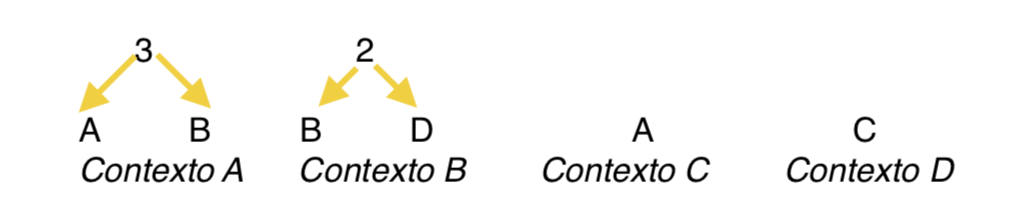
\includegraphics[width=8cm]{resumen-parcial-marijuan-ejemploOrdenSuperior}

El resultado obtenido es A00101000\\
La primera letra no está comprimida. Como es una A se que el siguiente caracter pertenece al contexto de la A. Como tengo un 0, entro al árbol del contexto de la A y me fijo cual es el 0. Luego vuelvo a tener una A, entonces el siguiente caracter pertenece al contexto de la A, y me fijo cual es el 0. De vuelta es una A, entonces, el siguiente caracter pertenece al contexto de la A, como es un 1 me devuelve una B y se que el siguiente caracter pertenece al contexto de la B. El siguiente caracter es un 0 entices según el árbol del contexto de la B ese 0 representa una B entonces el siguiente caracter pertence al contexto de la B.\\
Si quisiera hacerlo dinámico $\rightarrow$ genero todos los contextos con todos los caracteres con frecuencia 1 (en cada contexto). Luego en cada paso actualizo el contexto.\\

\textbf{Problema de la frecuecia cero}: Los métodos estáticos y dinámicos necestian archivos más grandes para funcionar con un orden cada vez mayor (ej. Al inicializar todo en frecuencia 1, el compresor necestiraría de un archivo muy grande para tener tiempo de aprender y comprimir eficientemente, no existen caracteres de frecuencia cero, porque si estos aparecieran, no se podrían representar). El hecho de aumentar el orden que se utiliza puede tener efectos negativos (la tabla de frecuencias se hace muy grande). Para solucionar esto, es necesario que el compresor sea dinámico ya que de lo contrario el peso de las tablas de frecuencias domina sobre el nivel de compresión que pueda alanzar el método. \\

\textbf{Compresor aritmético:} es capaz de comprimir los mensajes de una fuente en una cantidad no-entera de bits y gracias a esta capacidad los compresores artéticos son optimos dada una cierta distribición de probabilidades siendo los que mejor aproximan a la longitud ideal de los códigos que es $-log_2(p_i)$. Pueden ser estáticos o dinámicos, como también pueden tener órdenes superiores. \\

Funcionamiento: \\
Modelo estático: toma un intervalo de [0,1] y lo subdivide según la frecuencia de cada caracter, obtenido previamente en una tabla de frecuencia.\\
Toma el primer caracter y subdivide el intervalo con la misma proporción de la tabla de frecuencias. Toma el siguiente caracter y subdivide su intevalo. Así sucesivamente hasta quedarse con un sólo intervalo del cual se queda con uno de los extremos. \\
Para descomprimir, toma ese número y se fija en qué intervalo está y emite el caracter de ese intervalo. Subdivide el intervalo y vuelve hacer lo mismo hasta que el archivo está descomprimido. \\

\textbf{PPMC FALTA COMPLETAR CON UNA EXPLICACIÓN}(prediction by partial matching) es un algoritmo que alcanza un excelente nivel de copresión y está basado en modelos de compresión aritmética pero resolviendo el problema de la frecuencia cero. La forma por el cual resuelve el problema de la frecuencia sero es: en lugar de usar un sólo modelo de compresión de orden n usa varios modelos desde orden n hasta orden -1. Cuando un caracter no aparece en el modelo en el cual se lo busca entonces el algoritmo emite un símbolo especial (escape) y pasa al modelo de orden inmediato inferior. En cada modelo se inicializa únicamente el escape y se van agregando símbolos a medida que estos son observados en el archivo a comprimir. El modelo de orden -1 es un modelo especial en el cuál se inicializan todos los caracteres más el siómbolo EOF ocn frecuencia 1, es decir con probabilidad 1/257 y de esta forma se garantiza que cualquier símbolo del archivo original puede ser encontrado en alguno de los modelos. 

PPMC es en esencia un compresor aritmético puesto que en cada paso subdivide el intervalo actual de acuerdo al modelo que toque usar y se queda con el subintervalo que corresponde al símbolo emitido.  Luego de emitir se actualiza el modelo el cual pasamos como en cualquier algoritmo de compresión dinámico. 

\textbf{Aspectos claves de PPMC:}
\begin{itemize}
\item Es necesario fijar un órden máximo. 
\item El modelo de órden -1 tiene todos los caraceres posibles más el EOF y nunca se actualiza. 
\item La frecuencia de ESC es igual a la cantidad de caracteres en el modelo. 
\item Sólo se actualizan los modelos que se utilizan y esto se hace luego de haber comprimido cada caracter. 
\item Se suelen usar contextos de orden 5 o 6 al comprimir. 
\item El escape está relacionado con la probabilidad de encontrar un símbolo nuevo en el modelo, es decir, que ocurra un caracter que aun no se ha visto para un cierto contexto. 
\end{itemize}

\textbf{DMC: dynamic markov compression}
Algoritmo basado en comprimir los datos bit por bit, a diferencia de PPMC que procesaba byte a byte. DMC usa un único contexto por cada bit a  comprimir. Por cada bit a comprimir DMC intenta predecir la probabilidad de que el bit sea 1 o 0 comprimiendo el mismo con compresión aritmética. \\
Los pasos son los siguientes: \\
\begin{itemize}
\item Calcular la probabilidad de que el próximo bit sea 1 o 0. 
\item Leer el próximo bit del archivo. 
\item Dividir el intervalo de acuerdo a la probabilidad calculada y el bit leído (compresión aritmética). 
\item Incrementar la probabilidad del bit leído en el contexto actual (Hacerlo despues de dividir el intervalo). 
\item En base al bit leído determinar el próximo estado. 
\item Volver a 1. 
\end{itemize}

DMC es un algoritmo muy interesante ya que con memoria infinita es capaz de generar el modelo completo bit a bit del archivo. Un punto a tener en cuanta es que para que el algoritmo aprenda el modelo es necesario procesar el archivo por lo que el tiempo de entrenamiento puede ser alto. \\

La construcción de un \textbf{modelo de markov byte a byte (PPMC) o bit a bit (DMC)} a partir de cual calcular la probabilidad del próximo caracter o bit  suele dar buenos resultados en cuanto a compresión. Esto quiere decir que esta es una buena forma de modelar el contenido de un archivo. \textit{El modelo generado luego de comprimir puede ser usado como modelo generativo para crear datos similares al que acabamos de comprimir}. Simplemente hay que empezar en algún estado al azar y luego realizar un random-walk por el grafo de Markov que se ha aprendido. El resultado es que tanto PPMC como DMC pueden, luego de ser entrenados, usarse para generar textos, música u otros tipos de archivo de forma aleatoria. Cuanto más parecidos sean estos archivos generados por el modelos a los archivos reales que podría generar un persona más cerca está el algoritmos de "entender" de qué se trata ese tipo de archivos. \\

\textbf{Familia LZ de compresores: }
Se basan en el principio de reemplazar secuencias repetidas en el archivo por punteros a la posición en el cual dichas secuencias fueron observadas previamente. Se basa en la suposición de que secuencias de caracteres previamente obser vadas pueden volver a ocuririr en el archivo. Cuando esto ocurre podemos reemplazar una cantidad enorme de caracteres por un simple puntero a la posición previa de la secuencia y su longitud. \\

Se puede generalizar el comportamiento de un compresor d e la familia LZ de la siguiente forma: \\
\begin{itemize}
\item Es necesario definir la longitud de un buffer ov entana que será en donde busquemos las repeticiones. Cuanto más grande el buffer mayor cantidad de repeticiones podemos encontrar, pero al mismo tiempo más tiempo podemos tardar en procesar cada caracter. 
\item Es necesario limitar el buffer o usar índicies para poder buscar rápidamente un string dentro del mismo. 
\item La velocidad de compresión en un lz depende de la táctica utilizada para buscar las repeticiones en el buffer y la longitud del mismo. 
\item El descompresor en todos los LZ es extremadamente rápido ya que sólo necesita reemplazar  las repeticiones por lo que haya en la posición del buffer indicado. \textbf{En general la velocidad de los LZ es imposible de derrotar}.
\item Cada repetición se reemplaza por símbolos que permiten al descompresor determinar la posición en buffer y la longitud de la repetición. 
\end{itemize}

\textbf{LZSS}: versión mejorada del LZ77. Usa un bit para distinguir repeticiones de no repeticiones. Cada vez que se comprime un caracter del archivo se busca hacia atrás hasta una cierta cantidad máxima de caracteres llamada ventana en búsqueda de repeticiones.  Si se  encuentra una repetición entonces se emite un bit seguido d el aposición de la repetición en la ventana y la longitud de la misma. Cuando no se encuentran repeticiones se emite un bit en 0 y luego el caracter en cuestión en 8 bits. \\

En principio entonces hay que fijar dos parámetros: \\
\begin{itemize}
\item La longitud de la ventana en la que se buscan repeticiones. 
\item La longitud mínima de un match (podría no tener sentido buscar match de longitud 1). 
\end{itemize} 
Caracterísitcas del algoritmo: 
\begin{itemize}
\item Cuando se encuentran matches, se pueden utilizar los caracteres de la ventana y también los caracteres que se están matcheando. 
\item Las posiciones de la ventana se enumeran de izquierda a derecha. 
\item \textbf{Las limitaciones en el tamaño de la máxima longitud representable y el tamaño de la ventana hacen que LZSS no sea un compresor adecuado para aproximarnos a la complejidad de un string y por lo tanto no es usable en el cálculo de la distancia normalizada de compresión. }.
\item La cantidad de bits que usamos para la posición define la longitud de la ventana de búsqueda (o viceversa) y la longitud en bits que usemos para la longitud del match define el máximo match posible. 
\end{itemize}

LZSS ilustra muy bien la diferencia entre modelar y codificar. El modelo se basa en aprovechar secuencias de caracteres previamente observadas y la codificación en este caso es un simple modelo binario. \\

El mecanismo de parsing (análisis) de LZSS es de tipo "lazy" es decir, que siempre que se encuentra con un match lo reemplazamos por un offset y una longitud. Esto no siempre es óptimo ya que podría ser mejor ignorar un match para luego encontrar un match más largo. \\

La solución a este problema es analizar en cada paso la codificiación de la posición actual y la siguiente y compararla con la codificación de un literal y lo que sigue eligiendo en cada paso la opción que menos espacio no socupe. A esto se lo llama flexible parsing. \\

\textbf{Deflate (LzHuf):} evolución de LZSS en donde se mejora \emph{la forma de codificar}. La modelización es idéntica a la de LZSS. \\

Para la codificación se utiliza un árbol de Huffman dinámico en donde conviven los 256 caracteres y además todas las longitudes posibles (desde Lmin a Lmax).  Este árbol se utilizará para codificar los caracteres literales cuando no haya un match y para las longitudes cuando sí lo haya.  Cada vez se emite un caracter literal hay que actualizar el árbol incrementando su frecuencia. Cuando hay un match se emite su longitud en base al código de la misma en el árbol y a continuación su posición en la ventana en una cierta cantidad de bits que se puede fijar mediante otro árbol de huffman o bien de forma fija. Luego se actualiza la frecuencia de la longitud del árbol y se sigue comprimiendo el resto de los caracteres. \\

Esto introduce mejoras respecto a LZSS. Ellas son:
\begin{itemize}
\item Ya no hace falta distinguir con un 1 o un 0 si se trata de un match o no. Cuando se emite un caracter no hay match y cuando se emite una longitud hay match. El descompresor sabe que si descomprime una longitud lo siguiente será un aposición mientras que si descomprime un literal lo siguiente es o bien un literal o bien una longitud (mismo árbol).  
\item Puede aprender cuáles son los caracteres literales más frecuentes en el archivo y usar menos bits para los mismos. Tambien se pueden aprencer cuáles osn las longitudes más frecuentes en los matches y usar menos bits para esta longitudes que para los que no son tan comunes. 
\end{itemize}

\textbf{LZW:} es una versión mejorada del algoritmo LZ78. Para reemplazar secuencias previamente observadas por un código  que las prepresente lo hace es utillizar una tabla odiccionario en donde va almacenando las secuencias previamente observadas en el archvo. De esta forma cuando encuentra alguna secuenia que ya vio simplemente la reemplaza por el índice de la misma en el diccionario o tabla. \\
Inicialmente, LZW comienza con una tabla de 512 posiciones en donde las primeras 256 entradas ya están llenas con las combinaciones posibles de 8 bits y las restantes de 256 posiciones están vacías. \\

Cuando la tabla se completa, el compresor duplica la tabla y comienza a emitir códigos de 10 bits en lugar de 9. Este proceso se repite tantas veces como sea necesario. \\

Puede prestar a confución en qué momento el compresor comienza a emitir símbolos de 10 bits. Esto puede ocurrir o bien cuando se llena la tabla o bien un símbolo más adelante. \\

LZW es el único de todos los algoritmos de compresión en el cual el compresor y el descompresor no van sincronizados perfectamente. \\
El compresor agrega a la tabla un nuevo símbolo luego de comprimir un caracter, el descompresor sin embargo sólo sabe cuál es el símbolo agregado por el compresor al leer el siguiente. \\

En el caso que el descompresor lea un código que todavía no completó lo que hace es completarlo sabiendo que el próximo a leer tendrá en su primera letra lo que le faltó por completar. \\

\textbf{Snappy:} Es una variante de LZ optimizada para comprimir y descomprimir con gran fvelocidad y esto se logra en sacrificio de la compresión. \\

En Snappy el primer byte de cada bloque indica en sus dos primeros bits el tipo de dato que sigue a continuación:
\begin{itemize}
\item 00 = literals
\item 01 = 1 byte match
\item 10 =  2 byte match
\end{itemize}
Literales: los siguientes 6 bits se usan para la longitud de los mismos de la siguiente forma: 
\begin{itemize}
\item 0 a 59: cantidad de literales 1 a 60. 
\item 60: la cantidad de literales se indica en el próximo byte (61 a 61 + 256). 
\item 61: la cantidad de literales se indica en los próximos dos bytes. 
\item 62: la cantidad de literales se indica en los próximos tres bytes. 
\item 63: la cantidad de literales se indica en los próximos cuatro bytes. 
\end{itemize}
Los matches de longitud 4 a 11 con offsets de 1 a 2047  se almacenan usando 1 byte extra.  La longitud del match menos 4 se almacenan en los primeros 3 bits de los 6 que sobran del byte de controlo. Los restantes 3 bits y los 8 bits del byte siguiente se usan para almacenar el offset. \\

En conclusión: el primer bit de cada byte indica si el número termina en dicho byte (0) o continua en el siguiente. Los restantes 7 bits tienen el número. \\

Para buscar matches Snappy usa una tabla de hash hasheando los 4 bytes que siguen a comprimir. \\

\textbf{LZMA:} es el algoritmo de la familia LZ que mejor nivel de compresión logra. A diferencia de los demas LZMA puede generar 7 códigos, ellos son:
\begin{itemize}
\item Un LITERAl representa simplemente un byte literal al igual que en LZSS. 
\item un MATCH es un match en el estilo de LZSS indicando su longitud y distancia en el buffer mismo. 
\item Shortrep es un match de longitud 1 cuya distancia es igual a la distancia anteior emitida. 
\item Longrep[i] es un mach cuya longitud se indica y cuya distancia es igual a la i-esima distancia anteriormente emitida, es decir, la última para Longrep[0], la ante-ultima para longrep[1] y así sucesivamente. 
\end{itemize}
LZMA usa compresión aritmética para codificar todos su símbolos. \\

LZMA usa un buffer de 4 gb y hashing para encontrar los matches, además usa optimal parsing analizando las diferentes opciones que tiene el compresor en cada paso y luego de ver algunos pasos hacia adelante selecciona la estrategia de compresión más conveniente. \\

FALTA AGREGAR CODIFICACIÓN ARITMÉTICA Y USO DE EXCLUSIÓN QUE NO LOS ENTENDÍ. 

\textbf{Block sorting:} La compresión de Block Sorting comprende 3 etapas:
\begin{itemize}
\item Aplicar transformación de Burrows y wheeler. 
\item Aplicar MTF.
\item Aplicar algún compresor estadísitico. 
\end{itemize}

\textbf{Archivos localizados y  MTF:}\\

Un archivo está localizado cuando en determinadas zonas del mismo hay preponderancia de un cierto conjunto de caracteres. \\

Un archivo localizado es una generalización de las secuencias repetidas, en cierta forma cualquier archivo con secuencias repetidas está localizado pero no cualquier archivo localizado tiene secuencias repetidas. \\

Cuando un archivo está localizado el algoritmo de MTF (move to front) nos permite representarlo eficientemente. El algoritmo es muy simple: cuenta con un vector de 256 posiciones que comienza con los 256 vectores posibles, por cada byte a procesar se emite el índice del mismo en el vector y luego se lo mueve al principio del mismo. \\

Siempre que el archivo esté localizado MTF va a disminuir su entropía. En el resultado de MTF predominan los caracteres bajos sobre los demás caracters y esto se lo puede aprovechar comprimiendo la salida del MTF con huffman o compresión aritmética.\\ 

\textbf{La transformación de Burrows y Wheeler:} permite tomar un archivo común no random y convertirlo en un archivo localizado. Funciona de la siguiente manera: \\
\begin{itemize}
\item Tomamos un archivo y lo dividimos en bloques de un cierto tamaño y construimos todas las rotaciones. 
\item Luego se ordenan las rotaciones del bloque alfabéticamente. 
\item El resultado de la transformación es la última columna de la matriz ordenada con un índice que indica en qué número de rotación queda el archivo original (Este número es muy importante para descomprimir). 
\end{itemize}
Para revertir la transformación lo que se hace es: 
\begin{itemize}
\item Se toma la palabra y y se ordenan los caracteres guardanto tambien la posición vieja de cara caracter. 
\item Se toma el número guardado (numéro de rotación en el que queda el archivo original) y se emite la letra que está allí. Con la posición vieja se va a una de las posiciones nuevas y se emite el caracter que está allí. Así sucesivamente. 
\end{itemize}
Una vez realizada la transformación de BW notar que como el archivo está localizado entonces es posible aplicarle MTF y finalmente codificar con Huffman o compresión aritmética. 

\section*{Hashing}

Veremos funciones de hashing para strings. \\

Al conjunto de claves posibles lo denominaremos "espacio de claves" y al conjunto de números que la función de hashing puede devolver lo llamaremos "espacio de direcciones". \\

Propiedades que debe cumplir una función de hashing: \\
\begin{itemize}
\item La función tiene que ser muy eficiente, es decir, generar el resultado en muy poco tiempo. El motivo por el cual usamos una función de hashing es para poder recuperar un dato de forma muy eficiente en tiempos imilar a O(1). 
\item La función tiene que producir la menor cantidad de colisiones posibles. Esto también quiere decir que debemos intentar que la distribución de claves en el espacio de direcciones sea lo más pareja posible.  
\end{itemize}

Algunas funciones de hashing óptimas para string son: 
\begin{itemize}
\item FNV
\item Jenkings
\item Pearson
\end{itemize}

\textbf{Funciones de hashing criptográficas:} aquellas que deben cumplir requisitos adicionales que hacen a la seguridad de las mismas. \\
\begin{itemize}
\item La función de hashing tiene que producir la menor cantidad de colisiones posibles. 
\item Dado h(x) tiene que ser muy difícil encontrar x. 
\item Tiene que ser muy difícil encotrar x e y de forma tal que h(x)=h(y). 
\item Un cambio mínimo en la clave tiene que producir un cambio significativo en el resultado. 
\end{itemize}

La eficiencia no es importante sino la seguridad. \\

No hay ningún escenario en donde se puedan intercambiar funciones de hashing. \\

La librería hashlib de Python es la que tiene las funciones de hashing criptográficas. \\

Funciones de hashing más populares: 
\begin{itemize}
\item sha256
\item md5 No se usa más porque se le encontraron colisiones. Una vez que se encuentran colisiones, se invalida la parte criptográfica. No es que no existan las colisiones, son más difíciles de encontrar. \\
\end{itemize}

\textbf{Hashing universal} \\

Consiste en construir , no una función de hahing, sino una familia de funciones de hahsimg, de forma tal que podamos elegir las funciones que necesitemos entre el total de funciones que constituyen dicha familia. 

H es una familia de funciones de hashing de la forma $h\ \epsilon\ H: u\rightarrow [0,..., m-1]$. Es universal si: $$\forall x, y\ \epsilon\ U, \ h \epsilon H, x \neq y $$ $$ P[h(x) = h(y)] \leq \frac{1}{m} $$

Es decir que para cualquier función de hahing de nuestra familia, la probabilidad de que dos claves diferentes colisionen debe ser menor o igual a $\frac{1}{m}$ siendo m el espacio de direciones de cada una de las funciones de hashimg de la familia. \\

\textbf{Hashing universal para valores atómicos (numéricos)}\\



\textit{Hashing universal para números: Carter-Wegman:} $$h\ \epsilon H \rightarrow h(x) = (a*x+b*mod(p)) mod(m)$$
En donde p es un número primo mayor o igual a m, a es un número entre 1 y p-1 y b es un número entre 0 y p-1. 

\textit{Hashing universal para strings de longitud fija:  }\\

En realidad no tiene que ser un string puede ser cualquier tipo de dato de longitud fija.   \\

Sea m un espacio de direcciones, p un número primo mayor igual a m, sea x una clave compuesta por r+1 elementos: $x_0, x_1 ..., x_r$ entonces r e la longitud de x.  Vamos a elegir r+1 números $a_i$, entre 1 y m-1. La función de hashing queda definida por:
 $$ h\ \epsilon H \rightarrow h(x) = \sum_{i=0}^{r} (a_i * x_i (mod(p)) mod(m)) $$ 
 Es una familia de funciones ya que con diferentes selecciones de $a_i$ creamos una función diferente. Como $a_i$ puede tomar un alor entre 0 y m-1 hay un total de $m^{r+1}$ funciones de hashing en nuestra familia. 
 
 
\textit{Hashing unciersal para claves de longitud variable:}\\
Nuestras claves tienen una longitud variable y no hay una longitud máxima definida. La función de hashing se define como: $$ h \ \epsilon H \rightarrow h(x) = h_{int} \sum_{i=1}^l(x_i*a^i) mod(p)$$
En donde p es un número primo grande, a es un número aleatorio entre 0 y p-1 y $h_{int}$ es una función de hashing, tomada de la familia universal que definimos anteriormente que recibe un número entre 0 y p-1 y devuelve otro número entre 0 y m-1 siendo m espacio de direcciones. \\

\textbf{Cuckoo Hashing}\\

Es un algoritmo basado en múltiples funciones de hashing. Cada función de hashing va a definir una posición alternativa para nuestro dato en una tabla de hash. El algoritmo de búsqueda es muy simple. El dato tiene que estar en alguna de las dos posiciones alternativa o no está en la tabla, es decir, O(1). \\

La inserción de un nuevo dato funciona de la siguiente manera: \\
\begin{itemize}
\item Almacenamos el datos en la  primera posición indicada por la función de hashing. 
\item Si ese lugar estaba ocupado, entonces, reubicamos el dato (el que estaba) en su posición alternativa, es decir, el que da su segunda función de hashing. \\
\item Repetimos el proceso hasta que no haya más datos por reubicar o entramos en un loop. 
\end{itemize}

Un mecanismo para detectar si es posible o no dar de alta un nuevo dato sin detectar un loop previamente es: construir un grafo en donde los nodos son posiciones de la tabla y las arista unen posiciones candidatas por la función de hashing. El grafo resultante tiene que ser un pseudo bosque (un conjunto de pseudo árboles, un pseudo árbol es quel que puede tener un ciclo pero no dos). \\

La nomenclatura que utiliza este algoritmo es: $C_{n,m}$ en donde n es la cantidad de funciones de hashing a usar y m es la cantidad de registros por bucket. \\

Con este algoritmo se pueden generar tablas de hash bastante compactas. \\

Una mejora puede ser guardar una clave que falló en un área de overflow o stash. Esto permite que la clave se almacene y que el método continue siendo eficiente. Con áreas de stash relativamente pequñass el método puede lograr una eficiencia muy importante. El costo que agrega es buscar las claves en el stash.\\

\textbf{The hashing trick} \\

Tiene otros nombres como "feature hashing" o " Hash kernels". \\

BOW (bag of words) cada texto se represetna mediante un vextor que tiene tantas dimensiones como palabras existen en todos los documentos. En cada posición indicamos cuántas veces aparece en el documento. Si aplicamos THT lo que sucede es que \textit{reducimos el tamaño de los vectores sin perder poder de representación} (Cabe destacar que como no todos los documentos tienen todas la palabras, estos vectores son muy dispersos. \\

THT se resume en, por cada documento: 
\begin{itemize}
\item Decidimos el tamaño del vector que representará al documento. 
\item Por cada palabra del documento aplicamos una función de hashing en la que el espacio de direcciones es el tamaño del vector. 
\item Incrementamos en 1 la posición indicada por la función de hashing. 
\item El vector final luego de procesar todas las palabras del texto es su representación. 
\end{itemize}

THT  tiene propiedes muy importantes que son: 
\begin{itemize}
\item es un método que preserva la naturaleza dispersa de los datos. Los vectores dispersos son mucho más sensillos de trabajar. 
\item Con alguna variante u otra, puede usarse como método genérico para representar cualquier tipo de dato. 
\item el efecto de las colisiones, puede ocurrir que dos "features" diferentes de nuestros datos originales colisionen en un mismo feature al representarlos mediante THT. Empíricamnete se ha mostrado que el efecto de las colisiones es mínimo y en muchos casos es incluso favorable, reduciendo el ruido del set de datos. Cuando el  efecto de las colisiones no es bueno podemos usar el método de Weinberger para mitigarlas. 
\end{itemize}

\textbf{Método de Weinbeerger y hash kernels}\\

En esta variante usaremos una segunda función de hashing que devuelve solamente dos valores posibles: -1 y +1 y usaremos este resultado para decidir si incremenatamos o decrementamos la dimensión indicada por la primer función de hashing. Con este método, el promedio de cada columna en nuestros vectores va a tender a cero. Además, se minimiza el efecto de las colisiones, ya que no siempre incrementamos cuando dos features difrentes colisionan. El efecto más interesante de éste método es que le producto interno entre los vectores en nuestra nueva representación es equivalente al producto interno entre los vectores en el espacio original, lo cual admite el uso de THT para crear Hash kernels en donde usamos el producto interno etre los neuvos vectores para estimar la semejanza entre dos vectores (a mayor producto interno más semejantes son los vectores).\\

\textbf{Teorema de Johnson y Lindenstrauss}
Permite justificar que \textbf{es posible trabajar con un set de datos en menos dimensiones que las que tiene originalmente.}\\

\textbf{Teorema:} para todo conjunto de n datos en d dimensiones y una sierta tasa de error $0<\epsilon <1$ existe un entero positivo k de la forma: $$ k = 4\frac{1}{\frac{\epsilon^2}{2} \frac{\epsilon^3}{3}} log(n)$$
y existe una proyección $f: \Re^d\rightarrow \Re^k$ que cumple: $$(1-\epsilon) ||u-v|| \leq ||f(u)-f(v)|| \leq (1+\epsilon) ||u-v|| $$\\


Lo que el teorema nos dice, en definitiva es que es posible representar los datos en una cantidad de dimensiones en el orden de O(log(n)), siendo n la cantidad de datos, de forma tal que las distancias en el nuevo espacio dimensional sean muy similares a las distancias entre los puntos en el espacio original. \\

JL nos informa de la existencia de una proyección pero no nos dice como generarla. Métodos para generar una matriz de proyección que cumpla con el teorema de JL. \\

\textbf{1º proyección:} una matriz A = dxk en donde cada elemento $A_{i,j}$ de la matriz surge de una distribución normal conpromedio 0 y desvío estandar 1.\\

\textbf{2º proyección:} Si partimos de un conjunto de n datos en d dimensiones y queremos proyectarlos a k dimensiones nuestra matriz de proyección es una matriz de dxk en donde cada elemento $r_{i,j}$ de la matriz es +1 con probabilidad 1/2 y -1 con probabilidad 1/2.  \\

Para realizar la proyección se calcula: $ x' = \frac{x^*M}{\sqrt{k}} $ es decir que multiplicamos  por la matirz de proyección y escalamos por la raiz de k. \\

\textbf{3º proyección:} la tercera proyección defije una matriz dispersa en donde 2/3  de sus elementos son ceros y los restantes se distribuyen equitativamente entre +1 y -1. $r_{i,j} = \sqrt{3}$ * +1 con probabilidad 1/6 o 0 con probabilidad 2/3 y -1 con probabilidad 1/6. la ventaja de la tercera proyección con respecto a la segunda o a la primera es que es computacionalmente más eficiente para efectuar los cálculos. \\

\textbf{The hashing Trick y el teorema de Johnson Lindstrauss: } Existe una relación directa entre esta matriz y el THT de acuerdo al método de Weingberger. Mediante éste método podemos crear una matriz de proyección en donde la primera dirección me da la posición en la fila de la matriz y la segunda me da el valor +1 o -1 que va en esa celda. Usar THT es equivalente a miltimplicar un vector por esta matriz.  Esta matriz es la matriz que hemos demostrado que preserva las normas y por lo tanto las distancias y los productos internos entre vectores. Entonces por el teorema de JL se justifica el uso de hashing para reducir la dimensionalidad de los datos. \\



\section*{LSH}
LSH (localy Sensitive Hashing) es una solución muy eficiente al problema de los vecinos más cercanos. Este problema no aplica sólo a algoritmos como KNN sino a una enorme cantidad de otros algoritmos que necesitan encontrar el punto más cercano o los k puntos más cercanos a un cierto punto de nuestro set de datos. \\

LSH: aplicar a los puntos una función de hashing de forma tal que los puntos que son parecidos (cercanos) colisionen. Debe procesar cualquier elemento de $R^d$  y devolver como resultado un número de bucket. \\

Si logramos construir esta función es entonces sensillo resolver el problema de los vecinos cercanos: dado un punto "query" aplicamos la función de hashin y accedemos al bucket de la tabla de hash indicado por la misma, luego calculamos la distancia entre nuestro punto "query"  y todos los puntos dentro del bucket devolviendo el más cercano o los k más cercanos según el caso. \\

Queremos que la función LSH tenga una alta probabilidad de encontrar buckets con puntos cercanos y baja probabilidad de encontrar puntos lejanos. Necesitamos entonces dos distancias y dos probabilidades, ellas son:
\begin{itemize}
\item d1 la distancia para la cual queremos que dos puntos sean similares. 
\item p1 la probabilidad de que la función LSh nos de una colisión si la distancia entre dos puntos es menor o igual a d1. 
\item d2 la distancia para la cual queremos que dos puntos no sean similares. 
\item p2 la probabilidad de que la función nos de una colisión si los puntos están a una distancia d2 o más. 
\end{itemize}

$$H(d_1, d_2, p_1, p_2)$$

En general fijamos d2 =  c*d1 para una cierta constante c y queremos que p1>p2. Cuanto mayor es la difrencia entre p1 y p2 mejor sera la funcón de LSH. Una forma de evaluar esto es:
$$\rho = \frac{log(\frac{1}{p_1})}{log(\frac{1}{p_2})}$$

De esta forma podemos comparar diferentes funciones LSH buscando maximizar el valor de $\rho$ de forma empírica. \\

La función mágica que cumple lo de antes se llama \textbf{Minhash}. Estas funciones cumple que la probabilidad de que dos claves colisionen dependa de la distancia entre las claves. \\

Condiciones que debe cumplir una función de minhash:
\begin{itemize}
\item La probabilidad de que dos claves colisionen debe depender de la distancia entre las claves.En una función de hashing convencional la probabilidad de que dos claves cercanas o distantes colisionen es la misma. 
\item La función debe ser monótona y continua. Necesitmas que a medida que las claves estén más cerca la probabilidad de colisionar sea mayor
\item Debe existir una forma eficiente de calcular la función. De lo contrario, que ande más rápido que fuerza bruta no nos aporta ninguna utilidad. 
\item Debe ser posible randomizar la función de forma tal de poder obtener muchos minhash diferentes para una misma clave. Esta condición hace a la necesidad de que cada minhash nos defina una familia de funciones a partir de la cual podemos generar muchos minhashes para la misma clave en caso de ser necesario. 
\end{itemize}

Si no podemos derivar de forma teórica la probabilidad de colisión en función de la distancia entonces es sencillo hacer una simulación en la cual generamos claves a distintas distancias y calculamos la tasa de colidión, repitiendo el experimento n veces y promediándolo. \\

Un minhash nos define entonces una familia de funciones de hashing en donde p1 y p2 dependen de la distancia entre las claves. Por lo tanto podemos escribir una familia genérica para cualquier minhash de la forma: 
$$ h(d_1,d_2,f(d_1),f(d_2))$$

Una vez que tenemos una función de minhash válida para la distancia que nos interese es posible apmplificar la familia de funciones de hashing creadas por dicho minhash de forma tal que obtengamos los valores p1 y p2 que necesitemos. Esto se logra mediante el método de amplificación. \\

\textbf{Falsos negativos}: objetos que son cercanos pero no recuperamos. \\

\textbf{Falsos positivos}: objetos que no son cercanos pero igual recuperamos. \\

$1-p_1 $\textit{ es la probabilidad de falsos negativos y} $p_2$ \textit{es la probabilidad de falsos positivos. }\\

\textbf{Reducción de falsos positivos:} Es posible reducir la cantidad de falsos positivos usando más de una función de minhash sobre la misma tabla. Si usamos r funciones de minhash en la misma tabla cada una de ellas nos dará como resultado un bucket. Los documentos candidatos surgen entonces de la intersección de los documentos que estan en los r buckets que visitamos. \\

SI la probabilidad de colisionar es p, entonces, la probabilidad de colisionar los r buckets es igual a $p^r$. \\

La cantidad de falsos positivos disminuye a valores tan bajos como querramos pero también aumenta la cantidad de falsos negativos. \\

El tamaño d la tabla de hashing influye en la cantidad de falsos positivos y negativos ya que si la tabla es pequeña pueden producirse colidiones entre elementos que no son similares. \\


\textbf{Reducción de falsos positivos:} reducir los falsos negativos implica poder recuperar más objetos. La idea consiste en usar más de una tabla de hashing. SI usamos b tablas de hahing entonces podemos considerar a los objetos candidatos a aquellos que aparecen en alguna de las b tablas.\\

Si la probabilidad de que dos claves no colisionen es p entonces la probabilidad de que dos claves no colisiones es 1-p y la probabilidad de que dos claves no colisinen en ninguna de las bandas b es $(1-p)^b$. Por lo tanto, la probabilidad de que colisionen en alguna de las b tablas es $(1-(1-p)^b)$. \\

La cantidad de falsos negativos disminuye al mismo tiempo que aumenta la cantidad de falsos positivos. \\

Si combinamos ambos métodos: 
\begin{itemize}
\item la cantidad de total de minhashes es b*r. 
\item la probabilidad de colisionar usando b tablas de hashing y r minhahes por tabla es: 
$$p_{b,r} = 1 - (1-p^r)^b$$
\end{itemize}

 La notación es:\\
 
$|Mh_1,Mh_2,Mh_3|Mh_4,Mh_5,Mh_6|Mh_7,Mh_8,Mh_9|$. Cada bloque anterior funciona como una compuerta and. Y cada barrita funciona como una compurta or. \\

\textbf{LSH para la distancia de Jaccard}\\

Desarrollaremos una función de minhash para documentos de texto basada en la distancia de Jaccard. \\

Shingles: todos los n-gramas de n caracteres. La selección del n depende de los datos. En general para los documentos de texto está entre 5 y 10. \\

La \textbf{semejanza de jaccard} entre dos documentos se define como: $$sj_(D1,D2) = \frac{D1 \cap D2}{D1\cup D2} $$ 

Es decir, el cociente entre la cantidad de shingles que los documentos tienen en común y la cantidad de shingles entre ambos documentos. \\

La \textbf{distancia de Jaccard} se define como: $$dj_(D1,D2) = 1-\frac{D1 \cap D2}{D1\cup D2}$$

Imaginemos ahora una matriz en la cual las filas son todos los shingels que exisen en nuestra colección y cada columna representa un documento, indicado con 1 o 0 según el shingle aparezca o no en el documento. Tomemos hora una permutación al azar de las filas de la matriz y consideremos en qué número de fila aparece el primer 1 en cada columna. A este número lo llamaremos "minhash" (MH). \textit{Cada documento tiene entonces un minhash asosciado. }\\

\textbf{La probabilidad de que el minhash de dos documentos coincida es igual a la semejanza de Jaccard entre ambos documentos. }\\

De aquí se desprende que comparar los minhashes de los documentos es una forma lógica de evaluar la semejanza entre ambos.  Un sólo minhash nos da muy poca granularidad para medir la semejanza entre dos docuemntos. SI sólo tenemos un minhash nuestras opciones se limitan a decir que los documentos son similares (el minhash coincide) o bien no lo son (el minhahs no coincide). \\

\textbf{La solución, por supuesto, es usar más de un minhash y luego analizar cuantos minhash coinciden usando esta medida como semejanza entre documentos. }\\

Para esto vamos a usar tantas funciones de hashing ocmo minhash querramos usar y vamos a construir una pequeña matriz que tiene tantas filas como documentos y tantas columnas como minhashes.  A continuación vamos a precesar documento por documento, extrayendo los shingles y hasheando cada shingle con cada una de las 4 funciones de hashing. Lo que hacemos es acutliazar la tabla siempre y cuando el valor de la función de hashing sea menor al valor existente en la tabla.\\

Para demostrar que el minhash calculado de esta manera es equivalente a la posición del primer uno en la columna de nuestra matriz de shingles y documentos (para probar que sigue siendo válido que la probabilidad de coincidencia entre dos minhash es igual a la semejanza de Jaccard entre los documentos), lo que hacemos es probarlo intuitivamente:  \\

El valor que nos devuelve la función se hashing para un hsingle lo podemos considerar igual al número de fila en la cual apareceria dicho shingle en una permutación al azar de la matriz. Por lo tanto, el valor mínimo de minhash es equivalente al número de fila en el cual aparecería el primer 1 de la matriz. \\

Los shingles que no aparecen en un documento directamente no se hashean. De esto se desprende que el espacio de direcciones de la función de hashing a usar para los minhash es igual o mayor a la cantidad total de shingles en nuestra colección. \\

\textbf{Minhash para la distancia angular}\\

Una métrica muy popular especialmente para textos y strings representados como vectores es la distancia angular (es la medida de la distancia aparente entre dos puntos u objetos expresada en unidades de arco, suponiendo al observador en el vértice del ángulo). El coseno entre los vectores sirve entonces como medida de semejanza. Dos vectores que tienen igual dirección tiene distancia angular 0 y coseno igual a 1 mientras que que vectores que pauntan en direcciónes opuestas tienen distancia angular 180 grado y coseno igual a -1.\\

El coseno entre dos vectores se calcula como: $$cos(\theta ) = \frac{XY}{|X||Y|}$$

A efectos de simplificar podemos normalizar todos los vectores de forma tal que tengan norma 1. Por lo tanto: $$ cos(\theta ) = XY $$
 
 En la práctica muchos métodos LSH basados en la distancia angular funcionan bien para la distancia euclideana. Esto no tiene ninguna justificación teórica sino que ismplemente funciona. Es por esto que los minhashes para la distancia angular son de particular importancia.\\ 
 
 Para aproximar la distancia angular usando LSH existen varios minhashes posibles que desarrollaremos a continuación. \\
 
 \textbf{El método de los hiperplanos:}  para generar un minhash válido para la distancia angular vamos a calular el producto interno entre nuestro vector y un vector aleatorio. Este vector aleatorio puede estar formado simplemento por los valores +1 y -1, ya que estos son suficientes para deffinir un hiperplano aleatorio. El valor del minhash va a ser 1 si el resultado del producto interno es positivo y -1 si el resultado es negativo. \\ 
 
 Si interpretamos el significado del minhash,  \textbf{la probabilidad de que dos vectores proyectados al azar sobre un hiperplano tengan diferente signo es igual al el ángulo entre ellos dividido por 180.} Cuanto más chico el ángulo más probable es que las proyecciones tengan igual sentido. Por lo tanto, la probabilidad de que los minhashes coincidan para dos vectores es: $1-\frac{\theta}{180} $ . \\
 
 Por lo tanto con un solo minhash el método de las proyecciones aleatorias nos define la siguiente familia de funciones LSH: $(d1, d2, 1-d1/\pi , 1-d2\pi)$ En donde d1 y d2 son las distancias angulares entre los vectores. \\
 
 En la práctica como cada minhash nos define un valor de $\pm 1$ podemos decir que cada minhash nos define un bit y calculamos un minhash de k-bits usando k hiperplanos aleatorios. De esta forma tenemos un minhash que puede devolvernos valores entre 0 y $2^k$, siendo este el valor de cada una de las b tablas de hash que vamos a usar. Notemos que mayor valor de k aumentarn los falsos negativos ya que necesitamos que los puntos estén del mismo lado de los k hiperplanos usados para que el valor del minhash coincida. \\
 
 \textbf{Voronoi Hashing}\\
 
 En Vonoroi hashing vamos a usar un conjunt de T vectores aleatorios en donde los elemnetos de estos vectores surgen de una distribución normal, es decir, T vectores gaussianos. Vamos a calclar el producto interno entre cada uno de estos vectores y nuestro vector query y nos vamos a quedar con el índice del vector que nos da el máximo producto interno como valor del minhash.  \\
 
Lo que esto método está haciendo geométricamente es distribuyend T puntos al azar sobre la hiper-esfera unitaria y luego comparando cuál es el punto más cercano al punto hasheado. \\

Es interesante destacar que si usamos solo 2 hiperplano T=2, el método de Vonoroi es idéntico al de los hperplanos usando como hiperplano al que bisecte los dos puntos elegidos al azar por Voronoi. En general Vonoroi con T = $2^k$ gaussianos es igual al método de los hiperplanos con k hiperplanos. 
 
 
\textbf{LSH para la distancia euclideana }\\

\textbf{Método de las proyecciones aleatorias}\\

Vamos a usar proyecciones aleatorias, en este caso los hiperplanos aleatorios surgirán de una distribución p-estable, una distirbuiciónnormal funciona perfectemente. Cada vector lo vamos a multiplicar por un hiperplano aleatorio para obtener un número. Y el número obtenido lo vamos a discretizar a un número de bucket divdidiendolo por un cierto parámetro w. El resultado obtenido es el número de bucket o de minhash para la distancia euclideana. \\

La fórmula para calcular el minhash es entonces:  $$ mh_i(x) = \left[ \frac{x*v_i +a}{w}\right] $$ Donde w es un hiper-parámetro que depende de los datos, a es un número entre 0 y w-1 y $v_i$ es un vector aleatorio de igual dimensionalidad que neustros puntos. \\

SI analizamos la probabilidad de que dos documentos sean similiares de acuerdo a la forma en que hemos derinido los minhashes  para la distancia euclideana obtenemos que: \\

Cuando la distancia entre dos puntos es menor a w/2 la probabilidad de que caigan en el mismo bucket es de 1/2. \\

Cuando la distancia es mayor a 2w  los puntos solo caen dentro del bucket si su ángulo es cercano a 90 grados. En concreto, si el ángulo es menor a 60 grados, los puntos nunca pueden estar dentro del mismo bucket. Por lo tanto podemos decir que la probabilidad es 1/3, ya que esto ocurre 1/3 de los ángulos posibles. \\

Por lo tanto nuestra familia LSH es de la forma: $$LSH(w/2, 2w, p \geq 1/2, p \leq 1/3)$$ 

\section*{Reducción de dimensiones:}

Cuando aumenta el set de datos utilizado para entrenar un algoritmo, se requieren más recursos para procesarlos. En algunas ocaciones se agregan más features de las necesarias para entrenar al algoritmo. Entonces, la \textbf{reducción de dimensiones} se encarga de buscar una representación más compacta. \\

\textbf{La dimensión de los datos es igual a la cantidad de features que tiene un set.} A medida que aumentan los features, la dimensión va creciendo y se requiere un mayor muestreo para entrear un algoritmo. Algo a destacar es que agregar o quitar features conlleva a que un algoritmo funciones mejor o peor y eso dependerá de qué algoritmo se utiliza y de los datos en sí. \\

El hecho de tener cada vez más featuresen un set de datos puede empeorar la performance de un algoritmo. \\

Los algoritmos de reducción de dimensiones sirven muchas veces para \textbf{reducir el ruido de un set de datos} filtrando los features ruidosos y devolviendo un nuevo set de features con menor cantidad de ruido. \\

Los algoritmos para manipular la dimensionalidad de los datos se puede dividir en: 
\begin{itemize}
\item lineales: SVD y PCA. 
\item no lineales: algoritmos para Manifold learning. 
\end{itemize}

\textbf{Compresión de imágenes:} las imágenes se pueden pensar como datos en un espacio de muchas dimensiones. La dimensión de sicho espacio se puede reducir utilizando algún algoritmo como svd o PCA, entonces, se pueden ahorrar los bytes ocupados por una imagen a costas de reducir su calidad dado que en cierta forma reducir dimensiones implica perder cierta información. \\

\textbf{SVD: descomposición en valores singulares}\\

$$ A = U*\Sigma V^T$$

Pasos para calcularla:
\begin{itemize}
\item Calcular los autovalores y autovectores de $A^tA$. 
\item La matriz $\Sigma$ se compone de la raiz cuadrada de $A^tA$ de forma diagonal y ordenada de forma descendiente. 
\item La matriz U se compone con los autovectores normalizados como columnas. 
\item La matriz V se puede obtener resolviendo el sistema $AV = U\Sigma$ sabiendo que $V^tV$ es la matriz identidad. 
\end{itemize}

\textbf{SVD reducida:} Los valores de $\Sigma$ estiran la base ortonormal compuesta por los vectores de U.  Estos valores pueden ser cero y la consecuencia que traen es que anulan ciertas componentes a la hora de realizar el producto matricial y de ahí surge el concepto de descomposición en valores singulares reducida.  Los r valores de autovalores que no son nulos coninciden con el rango de la matriz.\\

La SVD da a entender que bajo determinados escenarios se podría encontrar una forma más compacta de representar la matriz A y esto da origien a la SVD para el uso de compresión de imágenes. \\

\textbf{Aproximación de rango k}
La SVD reducida de una matriz A se puede representar de una forma compacta donde utilizábamos aquellos r valores singulares no nulos puesto que eran los únicos que aportaban infomación, entonces permitía eliminar algunos valores de U y V. \\

Se puede pensar que como los valores de $\Sigma$ estan ordenados de mayor a menor entonces estos valores representan un grado de importancia de los datos. Esto podría dar a aentender que la matriz V es una base n donde los vectores de la base están ordenados por su grado de importancia. \textbf{En consecuencia, podría irse más allá de qudarse con los r valores no nulos, es decir opdría ser posible quedarse con los k valores no nulos siendo $k>r$ y aproximar bastante bien la matriz A. }\\

Para distintos valores de k podemos aprosimar mejor o peor la matriz A. Para saber que valor de k utilizar se define \textbf{la energía}: $$\sum_{i=1}^{n} \sigma_i^2$$
Donde n es la cantidad total de datos. Se puede obtner una fracción dividiendo la energía de k valores con la energía total. Se analizan los saltos de energía.  Si se utilizan todos los valores sigulares la energía es de 100. \\

El hecho de quedarnos con los vectores más importantes hace que se reduzca el \textbf{ruido del set de datos. } \\

\textbf{Eigen pictures:} Si cada columna es una imagen una svd de k valores se queda con las k más representativas. \\

Se puede aplicar para el reconocimiento de rostros de la siguiente manera: Por cada rostro a almacenar y que se quiere reconocer se almacena la distancia euclidiana del mismo a cada vextor de los eigenfaces, es decir, se obtendrán k distancias. De esta forma cada rostro qued a almacenado en una base de datos como un simple vector de k componentes. Cuando se quiere reconocer un nuevo rostro se calculan sus k componentes y se busca en la base de datos a ver si existe un rostro cuya semejanza de los k factores sea muy similar a la que se quiere reconocer y en base a esto se decide si tenemos un rostro que ya se ha capturados, un nuevo rostro o una imagen que no es un rostro. Esto último se puede calcular mediante la diferencia entre los k valores de la nueva imagen y un promedio de los eigenfaces. \\

\textbf{PCA: principal comonent analysis}\\
(es indentico a svd)\\

La ida es encontrar las "direcciones" principales de los dtos, es decir, aquellas dicrecciones sobre las cuales podemos proyectar los datos reteniendo su variablidadad. \\

Los ejes que devuelve PCA se llaman \textit{componentes prinipales}. Luego los datos se podrán pryectar sobre estas componentes logrando una reducción de dimensiones. Pasos para aplicar PCA a una matriz A.
\begin{itemize}
\item  para cada elemento de la columna i, restarle el promedio de dicha columna. Esto permite ccentrar los dtos en el origen. 
\item Para cada elemento de la columna i, dividirlo por la desviasión estándar de dicha columna. Esto permite escalar los datos. 
\item obtener la matriz de covarianza: $cov(A) = \frac{1}{n-1} A^t A$ 
\item Calcular los autovalores y autovectores de la matriz de covarianza. Los autovectores conformarán las componentes principales y los autovalores indicarán la importancia de cada componente. 
\end{itemize}

La matriz de covarianza es simétrica y en cada celda indica la covariancia entre las coumnas i y j de nuestra matriz original. CUando la covariancia es cercana a 0 las columnas son independientes y cuando la covariancia es cerca a 1 o -1 las columnas son dependientes. EN el caso concreto de la covariancia igual a 1 o -1 una columna es una combinación lineal de la otra y esto quiere decir que una de ellas es redundante. \\

Es interesante remarcar que para reducir las k dimensiones se pueden tomar las k componentes principales más importantes y proyectar los puntos de la matriz previamente normalizada sobre estas k ocmponentes principales reduciendo así las dimensiones. \\

\textbf{Conclusión:} la SVD es en general más eficiente y numéricamente más estable que PCA dado que no hace falta consturir la matriz de covariancia y es por este motivo que como método genérico lineal para la reducción de dimensiones se prefiere usar siempre la SVD.\\

\textbf{MDS: multidimensional Scaling}\\

Este algoritmo intente resolver el problema siguiente: dada una matriz de distancias entre puntos queremos  hallar los puntos en sí. Para poder aplicar éste algoritmo se debe realizar lo siguiente: 
\begin{itemize}
\item Elevar la matriz de distancias al cuadrado.
\item Centrar la matriz para que las filas y columnas tenga promedio cero. 
\item Calcular la SVD de la matriz. 
\item Las primeras q colunas de U da las cordenadas para los puntos que se quieren buscar. 
\end{itemize}

Las cordenadas que devuelve MDS pueden estar espejadas y rotadas con respecto a la realidad ya que las distancias en todos los casos son las mismas.\\

\textbf{Perceptual mapping:} es una aplicación interesante de MDS para aprender los datos a partir de evaluaciones subjetivas u objetivas de los mismos. Con la opinión de muchos usarios sobre si son parecidos o no paes de objetos que queramos comparar se puede construir una matriz de distancias. Luego, usando MDS, a partir de las distancias se puede construir una representación vectorial para cada modelo de auto en una cierta cantidad de dimensiones. Cada una de estas dimensiones va a aparotar algun tipo de información de cada objeto. Se puede ver que para cada "feature" cuál es el valor que toma cada objeto y deducir cuál es el feature. Lo que se está haciendo es una cosntrucción de los datos mismos a partir de las comparaciones entre objetos. \\

\textbf{ISOMAP: } es un algoritmo de Manifold Learning no lineal. Consite en construir un grafo a partir de los datos, calcular las distancias en dicho grafo y luego aplicar MDS para obtener una representación de los datos en pocas dimensiones. \\

\textit{Construcción del grafo:} crear un grafo no dirigido en donde cada punto del set de datos va a estar ocnectado a sus k vecinos más cercanos. Para determinar las distancias se puede usar una métrica a elección. En el grafo dos puntos i,j estarán conectados si j está entre los k vecinos más cercanos de i o viceversa. La matriz del grafo tendrá en cada posición la distancia y será muy disperso ya que tiene k vecinos. \\

\textit{Cálculo de las distancias:} una vez obtenido esto se construye una nueva matriz de distancias de todos los puntos contra todoos palicando el algoritmo de Floyd-Warshall. Es O($n^3$).\\

Una vez obtenida esta nueva matriz  de distancias de todos los puntos contra todos, simplemnete se aplica MDS con k = 2 o k =3 para obtener representación de los puntos en 2 o 3 dimensiones respectivamente. \\

\textbf{Laplacian Eigenmaps:}\\

En este algoritmo también se crea un grafo a partir d elos datos pero de una forma diferente a la que se utilizó en ISOMAP. \\

Para la construcción del grafo es encesario construir una matriz de adyacencia en donde cada nodo va a estar conectado con sus k vecinos más cercanos y el peso de las aristas entre nodos vecinos estará dado por la siguiente fórmula:  
$$ W_{i,j} = e^{-\frac{||x_i - x_j}{\sigma}} $$ El parametro $\sigma$ regula el radio al rededor del cual dos puntos se consideran vecinos. W es una matriz de adyacencias pero no de distancias. Cuanto  más grande el valor de $W_{i,j}$ más cercans osn los puntos. \\

El laplaciano se construye de la siguiente manera: L = D-W. \\

En donde D es una matriz diagonal con el grado de cada vértice del grafo siendo el grado la sumatoria de todas la arsitas que inciden sobre el mismo, es decir que Dii es la suma de todos los pesos que inciden sobre el mismo. \\

La matriz L tendra en su diagonal el grado ya que la diagonal de W es ero. El resto de los elementos de L es igual a la matriz W cambiada de signo.  La suma de cualqueir fila y lolumna de L es cero. Siendo L una matriz simétrica sabemos que todos sus autovalores son reales. El último paso del algoritmo es descomponer L en sus autovalores y autovectores. \\

\textbf{TSNE} es el mejor algirmto para la representaión de datos en dos y tre dimensiones. TSNE a difrencia de PCA y al igual que en Laplacian Eigenmaps, va a intentar qu elos puntos que están cerca en n dimensiones se mantengan cercanos en k dimensiones. \\

\textbf{Teorema fundamental de la dimensionalidad:} no siempre es conveniente reducir la dimensionalidad de un set de datos. \\

Cuando se trata de visualización TNSE es un buen algoritmo para empezar. 

Si se trata de reducir las dimensiones por cuestiones de performance o pra mejorar el rendimiento de un algoritmo la SVD debería er la primer opción teniendo en cuenta la posibilidad de usar algoritmos más avanzados. \\


\section*{Information Retrival}

Sección de la informática que se ocupa de recuperar infor de las computadoras, es decir, hacer consultas sobre infomación almacenada. \\

\textbf{Dominio: } conjunto de documentos. \\
\textbf{Documento:} compuesto de términos. Pueden ser TXT o páginas de internet. \\

\textbf{Consulta puntual:} consiste en recuperar todos los documentos que contienen una determinada palabra. Para colección de un tamaño mediano a grande necestiamos alguna estructura de tipo índice que nos permita resoler la consulta sin recorrer todos los documentos. \\

\subsection*{Indice invertido (II)}

Un índice invertido ocontiene por cada palabra una lista de documentos de donde la palabra aparece. \\

\textbf{Estructura de un índice invertido: }\\
\begin{itemize}
\item Léxico: lista de terminos. 
\item Punteros: número de documento donde ocurren los términos. 
\end{itemize}

\textbf{Técnicas para almacenar el léxico:}\\

\textbf{Léxico concatenado:} 
\begin{itemize}
\item Todos los términos concatenados uno al lado del otro. 
\item Tabla en donde en cada posición almacenamos el offset a donde está almacenado el término. 
\item Cuando llegamos a la posición de esta tabla leemos la posición siguiente para saber la longitud del término. 
\item Comparamos con el que buscamos. 
\end{itemize}

\textbf{Front coding:} se utiliza en casos en los que se quiere comprimir más el léxico. En la esturctura indicamos: 
\begin{itemize}
\item La cantidad de caracteres compartidos con el término anterior. 
\item antidad de cara teres diferentes. 
\item Puntero a esos caracteres. 
\end{itemize}

Para poder hacer una búsqueda binaria, al front coding, lo dividimos en bloques. No continuamos con verificar cuanto comparte con el anterior infinitamente. \\

Usamos front coding cuando buscamos rapidez o tenemos poca memoria. \\

Cuando tenemos memoria suficiente y queremos acceder muy rápidamente a un término podemos prescindir de la búsqueda binaria y usar por ejemplo una tabla de hash para recuperar los términos, si la colección es estática que frecuentemente e s el caso podemos usar hashing perfecto para acceder a cada término en O(1). En otros casos podemos usar tablas de hash enormes de forma tal de minimizar las colisiones usando algún método de resolución de colisiones que hemos visto. \\

\textbf{Almacenamiento de punteros a doc:}\\
\begin{itemize}
\item \textbf{Trivial:} cada puntero es un número de documento. 
\item \textbf{Almacenar la distancia:} de esta manera reducimos la entropia. El problema persiste porque la distancia máxima sigue siendo el  número de documento. 
\item \textbf{Almacenar los número con longitud variable:} indicar en el primer bit si el número sigue en el próximo byte. 
\item \textbf{Almacenamiento de punteros final: } concatenar distancias uno atrás de la otra usando una estructura de longitud variable. 
\end{itemize}

\textbf{Conexión entre léxico y punteros: } usamos el almacenamiento de punteros final. En el léxico debemos agregar un puntero al offset donde empiezan los punteros a documento (el término siguiente nos dice donde detenernos). \\

\textbf{Almacenamiento de punteros: } Sabiendo que las distencias pequeñas son las mas frecuentes buscaremos comprimirlos. Las maneras de almacenar punteros son: 
\begin{itemize}
\item \textbf{Código unario:} n-1 bit en 0 y luego un sólo 1. Para la distancia n el código unario ocupa exactamente n bit. Tiene la \textbf{propiedad} que se pueden almacenar uno atrás del otro sin separadores o longitudes. Es eficiente para distancias pequeñas. Buscaremos que todas nuestras codificaciones cumplan con esta propiedad. 
\item \textbf{Código gamma:} escribimos $log_2(x) +1$ en unario. Luego le concatenamos $x-2^{log_2(x)}$ en binario de $log_2(x)$ bits (Para codificar más fácil, lo que puedo hacer es escribir el número en binario y luego le agrega
al principio una cantidad de ceros equivalente a los dígitos del número en binario menos 1). 
\item \textbf{Código delta:} un código delta es igual a un código gamma con la salvedad de que la parte que en gama se escribía en unario en delta se escribe en gama. 
\end{itemize}

\textbf{Consulta de frases o proximidad entre términos:} tenemos que modificar nuestro índice invertido agregando información sobre la posición en la que ocurren las palabras en los documentos. Debemos codificarlos con códigos gamma o delta. \\

\subsection*{Signature files} 

Se usa cuando no se puede usar II por no haber espacio suficiente. Usamos funciones de hashing para obtener una representación de cada documento. Representamos mediante hashing cada término. Necesitamos k funciones cucho espacio de direcciones sea de b bits. El signature consiste en prender los bits indicados por las funciones de hashing para cada palabra. El signature de un documento es el resultado de realizar un or entre los signatures de sus términos.\\

\textbf{Bit slices: }Mejora al signature files. En vez de almacenar los documentos uno abajo dle otro, los almacenamos en vertica y buscamos las filas que deben estár encendidas. No accedemos a todos los documento sen una sóla búsqueda. \\

Para que SF funcione la cantidad de 0 y de 1 debe ser pareja. Muchos 1 da falsos positivos. \\

\subsection*{Bit maps}

Es una forma de índice muy particular y que ocupa mucho espacio a menos que esté comprimida. Se guarda un vector de N bit por cada término (N es la cantidad de documentos). Se guarda un 0 o un 1 según se encunetre en el documento. Tiene la particularidad que el bitmap comprimido puede usarse para hacer consultas sin necesidad de reconstruirlo completamente. \\

\textbf{Consultas rankeadas:} obtener una lista de documentos más relevantes para la consulta ordenados por relevancia. Consulta: lista de términos. Formas de resolverlo: 
\begin{itemize}
\item Producto interno entre la consulta y el vector del documento (BOW). 
\item Resolver por indice invertido, recuperamos los documentos para cada término de la ocnsulta y luego vemos qué documento tiene más puntaje. 
\end{itemize}

\textbf{TF-IDF:} Mejoras para identificar términos más importes. TF (term frecuency): contar la cantidad de veces que parece cada término de la consulta en cada documento. IDF darle a cada término un peso que sea inversamente proporcional a su frecuencia. Los términos que parecen en muchos docuemntos serán menos imortantes que los que aprecen en pocos. $$IDF(t_i) = log(\frac{N+1}{fti}$$ en donde N es la cantidad de documentos y $ft_i$ es la cantidad de documentos en los que parece cáda término.\\

Por cada término de la consulta y cada documento multiplicamos el valor de TF por IDF y eso noe sda el peso del término para ese documento. El puntaje del coumento es la sumatoria del puntaje TF-IDF de todos los términos de la consulta que aprecen en el documento. $$R(Q, D_j) = \sum_{t_i \epsilon Q, t_i \epsilon D_j} ft_{i,j} log( \frac{N+1}{ft_i}) $$donde $ft_{i,j}$ es la frecuencia del término i en el documento j es decir cuántas veces aparece. \\

Surge un nuevo problema que es que TF tiene mucho peso en el ranking. Para resolverlo modificamos la manera de calcular la frecuencia del término en el documento:  \textbf{BM25}: se define $$TF_{i,j} = \frac{(k+1)ft_{i,j}}{ft_{i,j}+k} $$ Cuando k = 0 es el modelo binario. Cuando k$\rightarrow \infty$ se trata del modelo lineal. Con k intermedios se aproxima a las variantes logaritmicas. \\

La formua de ranking con la transformación BM25 queda de la forma: $$R(Q, D_j) = \sum_{t_i \epsilon Q, t_i \epsilon D_j}  \frac{(k+1)ft_{i,j}}{ft_{i,j}+k}log( \frac{N+1}{ft_i}) $$

Surge un nuevo problema que es: los documentos largos tienen ventaja sobre los documentos cortos. La solución es \textbf{Normalizar docuemntos según la longitud.}  $$norm_j = 1-b+b\frac{|D_j|}{avdl} $$ en donde $b\epsilon [0,1]$. Cuando b=1 la normalización penaliza a los más largos. Cuando b = 0, no hay normalización. b: rango de penalización. Entonces la función del ranking queda así: 

La formula de ranking con la transformación BM25 queda de la forma: $$R(Q, D_j) = \sum_{t_i \epsilon Q, t_i \epsilon D_j}  \frac{(k+1)ft_{i,j}}{ft_{i,j}+k (1-b+b\frac{|D_j|}{avdl})}log( \frac{N+1}{ft_i}) $$

\textbf{Indexación semántica latente: LSI}\\

Consiste en aplicar SVD a la matriz de términos por documento ($A_{i,j}$ = peso del término i en el documento j, se calcula por TFIDF o BM25). \\

Con esta matriz podemos resolver consultas mediante el método del coseno. Este método consiste en  calcular el coseno entre el vector  y el vector documento. Si normaliamos es el PI.\\

LSI: consiste en descomoner la matriz de documentos por términos aplicando SVD y quedarnos con las k primeras columnas de la matriz U. \\

\textit{Al calcular la SVD estamos decomponiendo cada documento en una combinación lineal de elemtnos de la base v donde cada vector de la base V es una combinación lineal de términos, llamemos a estos vectores, entonces, conceptos. Al quedarnos con las primeras columnas de U estamos representando cada documento en los k conceptos más importantes. }\\

Para poder realizar una consulta es necesario plegar elvector consulta al nuevo espacio de dimensiones, esto lo sabemos hacer e involucra multiplicar al vector consulta por V y $\Sigma^-1$ esto nos da la representación de la consulta Q en k dimensiones que podemos usar para calcular el producto interno contra cada uno de lso vectores de los documentos para luego ordenarlos por puntaje. Una consecuencia favorable es que al ser vectores más chicos el proceso es más eficiente. 
\end{document}